\NeedsTeXFormat{LaTeX2e}
\documentclass[11pt]{article}
%Absaetze nicht einruecken:
\usepackage{parskip}
\usepackage[utf8]{inputenc}
\usepackage[T1]{fontenc}
\usepackage{ae}
\usepackage[intlimits, sumlimits, namelimits]{amsmath}
\usepackage{bbm}
%Neue Macros fuer Mathe:
%in parentheses - gleich mit richtiger Groesse
\newcommand{\inp}[1]{\ensuremath{\left(#1\right)}}
\newcommand{\sqr}{\ensuremath{^{2}}}
\newcommand{\cube}{\ensuremath{^{3}}}
%Mengensymbole mit doppelten senkrechten Strichen:
\newcommand{\set}[1]{\ensuremath{\mathbbm{#1}}}
%definiert eine Norm, also zwei senkrechte Striche auf jeder Seite:
\newcommand{\norm}[1]{\ensuremath{\left|#1\right|}}
%Spaltenvektor - dreidimensional:
\newcommand{\svec}[3]{\ensuremath{\inp{\hspace{-.8ex}\begin{array}{r}#1\\#2\\#3\end{array}\hspace{-.4ex}}}}
\newcommand{\entspr}{\ensuremath{\,\,\hat{=}\,\,}}%
\newcommand{\dx}[1][x]{\ensuremath{\textnormal d #1}}

% For stupid thinkos:
\newcommand{\cross}{\times}

% Tabellen:
\usepackage{array}
\setlength{\extrarowheight}{.2mm}
%Links im Text:
\usepackage{hyperref}
\usepackage{graphics,graphicx,fancyvrb}
%Raender einstellen
%\usepackage[a4paper, margin=15mm, top=30mm]{geometry}
\usepackage[a4paper]{geometry}
%Kopf - und Fusszeilen
\usepackage{lastpage}
\usepackage{fancyhdr}
	\lhead{Moritz Lenz}
	\chead{\bfseries{-- \thepage\ --}}
	\rhead{\thetitle}
	\lfoot{}
	\rfoot{}
	\cfoot{}
	\pagestyle{fancy}
\pagestyle{empty}

\sffamily

%Kopfzeile

\author{Moritz Lenz}
\title{Adaption between chiral and spin up/down bases}
\begin{document}
\maketitle

The chiral spin bases are very natural for the analytical calculation, because the
base vectors are also eigenstates to the Hamiltonian.

However for the numerical simulation they are not suited, because they are
dependent on the direction (in real space) in which the wave travels. This
that's not known before the simulation runs, and because there can be several
waves with different directions in one place, it is not possible to calculate
the self-energy of the leads in these bases.

\begin{figure}
    \begin{center}
    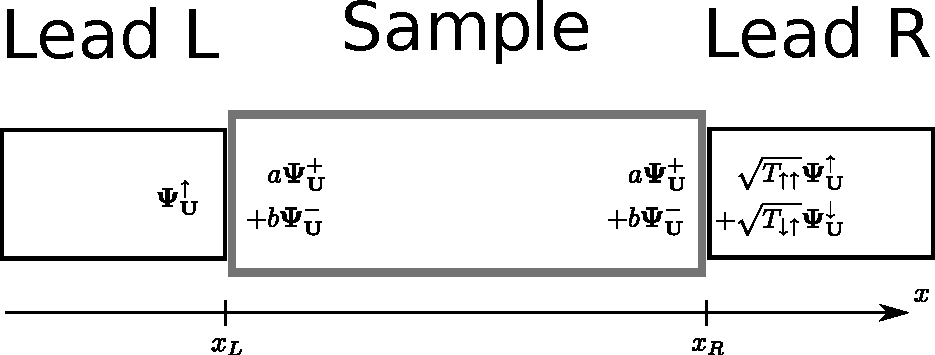
\includegraphics[width=0.8\textwidth]{adapting-pic.pdf}
    \end{center}
    \caption{Adapting the bases at the interfaces between leads and sample}
\end{figure}

Since there is no dissipation in our model, and we assume that the mere
process of injecting an electron doesn't change its spin, we know that

\begin{align*}
    |\uparrow> + |\downarrow> = a |\chi_N^+> + b |\chi_N^->.
\end{align*}

This is an equation in two components with two variables which let us
determine $a$ and $b$ unambiguously.

With probability $C_{++} = t_{++} \frac{v_+}{v}$ an electron in
the $\chi_N^+$ state is reaches the
\textbf{R} lead in the $\chi_{SO}^+$ state, and with the probability $C_{+-}$
into the $\chi_{SO}^-$ state and so on. So the total transmission is 

\begin{align*}
   T_{tot} =  a C_{++}|\chi_{SO}^+>
            + a C_{+-}|\chi_{SO}^->
            + b C_{--}|\chi_{SO}^->
            + b C_{-+}|\chi_{SO}^+>
\end{align*}

On the other hand the numerical simulation also provides us with a
transmission matrix, here the total transmitted current is 

\begin{align*}
	T_{tot} = T_{L+R+} |\uparrow>
              T_{L+R-} |\uparrow>
              T_{L-R-} |\downarrow>
              T_{L-R+} |\downarrow>
\end{align*}

where $T_{L+,R-}$ is the probability that an electron with spin up, injected from
the \textbf{R} lead, is transmitted into the \textbf{L} lead with spin down.

Comparing these two expressions for $T_{tot}$ we obtain another two-component
equation,

\begin{align*}
      a C_{++}|\chi_{SO}^+>
    + a C_{+-}|\chi_{SO}^->
    + b C_{--}|\chi_{SO}^->
    + b C_{-+}|\chi_{SO}^+>\\
	 = T_{R+L+} |\uparrow>
       T_{R+L-} |\uparrow>
       T_{R-L-} |\downarrow>
       T_{R-L+} |\downarrow>
\end{align*}

Each component of that equation can be calculated both analytically and by the
simulation, giving us a way to compare the two methods.

\end{document}

% vim: ts=4 sw=4 expandtab spell spelllang=en_us
